\setcounter{section}{4}

\Needspace{5\baselineskip}
\hypertarget{dqnux7b97ux6cd5}{%
\section{DQN算法}\label{dqnux7b97ux6cd5}}

\Needspace{5\baselineskip}
\hypertarget{ux4e00ux57faux672cux601dux60f3}{%
\subsection{一、基本思想}\label{ux4e00ux57faux672cux601dux60f3}}

在Q-learning算法中，我们以矩阵的方式建立了一张存储每个状态下所有动作Q值的表格。然而，这种用表格存储动作价值的做法只在环境的状态和动作都是离散的，并且空间都比较小的情况下适用。当状态或者动作数量非常大的时候，或者当状态或动作连续的时候，用这种表格形式来记录各个状态动作对的Q值是不现实的。我们需要用函数拟合的方法来估计Q值，即拟合一个函数Q(s,a)。

我们建立一个神经网络（函数），其训练目标是学习、拟合Q函数（可以形象理解为``Q地图''，不过实际上机器学习优化得出的是一个连续的函数）。输入是状态s（实际上是输入s对应的所有（状态s，动作a）对），输出是状态s对应的每种动作a的Q(s,a)的值（以实现在给定状态s下基于价值函数Q最大化的输出选择）。如训练一个多层感知机来拟合Q函数。

\begin{figure}[htbp]
\centering
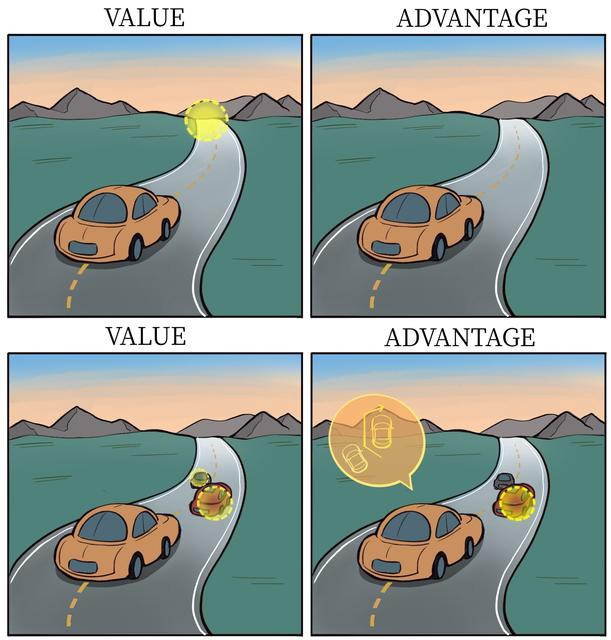
\includegraphics[width=0.82\linewidth]{images/image-0014.jpeg}
\caption{DQN 用神经网络拟合状态到各动作 Q 值的映射}
\end{figure}

\Needspace{5\baselineskip}
\hypertarget{ux4e8cdqnux7684ux635fux5931ux51fdux6570}{%
\subsection{二、DQN的损失函数}\label{ux4e8cdqnux7684ux635fux5931ux51fdux6570}}

\Needspace{5\baselineskip}
在传统的 Q-Learning 中，我们维护一张 \(Q\) 表。对于状态 \(s\) 和动作 \(a\)，更新规则如下：

\[
Q(s,a)\leftarrow Q(s,a)+\alpha\cdot\left[\left(r+\gamma\max_{a'}Q(s',a')\right)-Q(s,a)\right]
\]

\begin{itemize}
\tightlist
\item
  \(r+\gamma\max_{a'}Q(s',a')\) 是 TD Target（目标值），即我们认为 \(Q(s,a)\) 应该接近的值。
\item
  \(Q(s,a)\) 是 Current Estimate（当前估计值）。
\item
  物理意义：将当前的 \(Q(s,a)\) 向目标值拉近一点（步长为 \(\alpha\)）。
\end{itemize}

在 DQN 中，我们用神经网络 \(Q(s,a;\theta)\) 来拟合 \(Q\) 值。我们需要定义一个损失函数 \(L(\theta)\) 来训练网络。DQN 采用的是均方误差（MSE），目标是让网络的输出 \(Q(s,a;\theta)\) 尽可能接近 TD Target。

\[
L(\theta)=\mathbb{E}\left[\left(r+\gamma\max_{a'}Q(s',a';\theta^-)-Q(s,a;\theta)\right)^2\right]
\]

其中 \(y=r+\gamma\max_{a'}Q(s',a';\theta^-)\) 是目标值，在计算梯度时被视为常数；\(\theta^-\) 是目标网络的参数。

\Needspace{5\baselineskip}
\hypertarget{ux4e09dqnux7684ux68afux5ea6ux66f4ux65b0}{%
\subsection{三、DQN的梯度更新}\label{ux4e09dqnux7684ux68afux5ea6ux66f4ux65b0}}

\Needspace{5\baselineskip}
将目标值记为 \(y=r+\gamma\max_{a'}Q(s',a';\theta^-)\)，则 DQN 损失函数的梯度为：

\[
\begin{aligned}
\nabla_\theta L(\theta)
&=\nabla_\theta\left(y-Q(s,a;\theta)\right)^2\\
&=2\cdot\left(y-Q(s,a;\theta)\right)\cdot\nabla_\theta\left(-Q(s,a;\theta)\right)\\
&=-2\cdot\left[\left(r+\gamma\max_{a'}Q(s',a';\theta^-)\right)-Q(s,a;\theta)\right]\cdot\nabla_\theta Q(s,a;\theta)
\end{aligned}
\]

\Needspace{5\baselineskip}
其中括号中的差值就是 TD Error \(\delta\)。参数更新规则（梯度下降）为：

\[
\theta\leftarrow\theta-\eta\cdot\nabla_\theta L(\theta)
\]

\Needspace{5\baselineskip}
代入梯度后得到：

\[
\theta\leftarrow\theta+\eta\cdot2\cdot\delta\cdot\nabla_\theta Q(s,a;\theta)
\]

对比来看，Q-Learning 直接修改 \(Q(s,a)\) 的值，增加量正比于 TD Error；DQN 修改的是参数 \(\theta\)，使 \(Q(s,a;\theta)\) 的输出值沿梯度方向变化，变化幅度同样正比于 TD Error。

\Needspace{5\baselineskip}
\hypertarget{ux56dbux7ecfux9a8cux56deux653e}{%
\subsection{四、经验回放}\label{ux56dbux7ecfux9a8cux56deux653e}}

\Needspace{4\baselineskip}
\begin{enumerate}
\def\labelenumi{\arabic{enumi}.}
\tightlist
\item
  概念
\end{enumerate}

监督学习中，我们往往假设训练数据是独立同分布的，在训练时每个batch也是随机采样的，保证了每个batch的梯度方向是对整个数据集梯度方向的一个无偏估计。但在马尔可夫决策过程（MDP）中，智能体产生的数据是一个时间序列轨迹：s\_0, a\_0, r\_0, s\_1, a\_1, r\_1,\ldots，状态s\_\{t+1\}直接依赖于s\_t和a\_t。这意味着数据高度相关，如果机器人在走迷宫，前一秒它在左下角，下一秒它大概率还在左下角附近。如果直接拿这些数据训练，神经网络会连续看到很多``左下角''的数据。数据是一个非平稳分布：随着策略pi的更新，智能体访问的状态分布也会发生变化，导致训练数据的分布本身就在变。当它极力优化当前连续片段的数据时，它会修改共享的权重，导致它``忘记''了之前在其他状态下学到的知识（和大模型推理过程中的``灾难性遗忘''亦是如此）。

因而我们引入经验回放：智能体与环境交互，每一步生成一个四元组e\_t = (s\_t, a\_t, r\_t, s\_t+1)，将这个e\_t存入固定容量的缓冲区中。在训练时刻t，我们每和环境交互一次，就从缓冲区中均匀若干次随机采样小批次的数据来进行梯度下降。

\Needspace{4\baselineskip}
\begin{enumerate}
\def\labelenumi{\arabic{enumi}.}
\setcounter{enumi}{1}
\tightlist
\item
  优点
\end{enumerate}

打破相关性：通过随机采样，一个 batch 内的数据可能包含3天前的数据、5分钟前的数据、刚刚的数据，使得这个batch的数据分布接近于智能体的全局历史分布，而不是当前局部的一段轨迹，近似满足了独立同分布假设。

提高数据利用率：在原始Q-learning中，数据用完即弃。训练DQN网络时，每次获取新数据后，让Loss下降到接近0往往需要多次梯度下降拟合中，一个样本存入缓冲区后，可能会被多次采样用于梯度更新。这极大地提高了样本利用率（因为获取环境数据的代价通常很高）。

\Needspace{4\baselineskip}
\begin{enumerate}
\def\labelenumi{\arabic{enumi}.}
\setcounter{enumi}{2}
\tightlist
\item
  与Dyna-Q中引入的``环境模型''的区别
\end{enumerate}

DQN不试图理解环境的运作机制，只是维护一个巨大的经验池，里面存储的是真实的元组(s\_t, a\_t, r\_t, s\_t+1)构成。每次更新参数时，从经验池中随机抽取一批曾经真实发生的数据，直接利用这些历史事实来计算损失函数并更新神经网络。

``环境模型''则维护一个函数，输入s\_t和a\_t，该函数会输出r\_t和s\_t+1。在更复杂的情境下，这个模型通常是一个神经网络。我们更新参数时，随机选择一个过去走过的(s\_t,a\_t)，但并不用过去在某一次真实发生的(r\_t,s\_t+1)，而是运用这个网络的输出值。这个函数（神经网络）具有泛化性，在高级版本中我们还可以让环境模型选择没有走过的(s\_t,a\_t)，模型可以根据学会的物理规律给出一个预测（这是经验回放做不到的，因为经验回放池里没有这一条数据），运用网络的输出值，让Q网络学习泛化性能。

\Needspace{5\baselineskip}
\hypertarget{ux4e94ux76eeux6807ux7f51ux7edc}{%
\subsection{五、目标网络}\label{ux4e94ux76eeux6807ux7f51ux7edc}}

\Needspace{5\baselineskip}
DQN 算法最终更新的目标是让Q(s,a)逼近r+gamma*maxQ(s',a')，由于TD误差目标本身就包含神经网络的输出，因此在更新网络参数的同时目标也在不断地改变，这非常容易造成神经网络训练的不稳定性。为了解决这一问题，DQN便使用了目标网络的思想：既然训练过程中Q网络的不断更新会导致目标不断发生改变，不如暂时先将TD目标中的Q网络固定住。为了实现这一思想，我们需要利用两套Q网络。对于损失函数：

\[
\frac{1}{2}\left[Q_w(s,a)-\left(r+\gamma\max_{a'}Q_{w^-}(s',a')\right)\right]^2
\]

原来的训练网络（主Q网络）Q\_w用于计算损失函数中的第一项，并且使用正常梯度下降方法来进行更新。目标网络Q\_w-用于计算损失函数中的第二项，其中w-表示目标网络中的参数。如果两套网络的参数随时保持一致，则仍为原先不够稳定的算法。为了让更新目标更稳定，目标网络并不会每一步都更新。具体而言，目标网络使用训练网络的一套较旧的参数，训练网络在训练中的每一步都会更新，而目标网络的参数每隔C步才会与训练网络同步一次，即。这样做使得目标网络相对于训练网络更加稳定。

当然，目标网络也不一定直接同步训练网络的值。也可以采取``软更新''：它不会大幅改动目标网络的参数，而是缓慢地将其向主Q网络的方向调整，每隔C步，计算w-\_new=τ\emph{w+(1−τ)}w-\_new。这确保了目标Q值相对稳定，为主Q网络提供了一个可靠的学习目标。

\FloatBarrier
\Needspace{5\baselineskip}
\hypertarget{ux53c2ux8003ux6587ux732e-50}{%
\subsection{参考文献}\label{ux53c2ux8003ux6587ux732e-50}}

\vspace{0.25em}
\begin{itemize}
\tightlist
\item
  \href{https://hrl.boyuai.com/}{《动手学强化学习》}.
\item
  Mnih, V., Kavukcuoglu, K., Silver, D., et al.~(2015). \href{https://www.nature.com/articles/nature14236}{Human-level control through deep reinforcement learning}. Nature.
\end{itemize}

\clearpage
